\documentclass{beamer}
\usetheme{PaloAlto}
\usepackage{graphicx}

\newtheorem{requirement}{Requirement}



\begin{document}



\title[LingSync \& OLD] % (optional, use only with long paper titles)
{LingSync \& the Online Linguistic Database}



\author[~]{Joel Dunham \inst{1} \and Gina Cook \inst{2} \and Josh Horner \inst{3}}
\institute[UBC, LingSync.org]{\inst{1} University of British Columbia \and %
                      \inst{2} iLanguage Lab \and %
                      \inst{3} Amilia}


\subtitle
{New models for the collection and management of data for language communities, linguists and
language learners}

%\author[Author1,Author2] % (optional, use only with lots of authors)
%{Author One  \and Author Two }
% - Give the names in the same order as the appear in the paper.
% - Use the \inst{?} command only if the authors have different
%   affiliation.

% - Use the \inst command only if there are several affiliations.
% - Keep it simple, no one is interested in your street address.

\date[ComputEL 2014] % (optional, should be abbreviation of conference name)
{ComputEL Workshop, June 26 2014}



% \AtBeginSubsection[]
% {
% \setbeamertemplate{sidebar left}{}
%   \begin{frame}<beamer>
%     \frametitle{Outline}
%     \tableofcontents[currentsection,currentsubsection]
%   \end{frame}
%   \setbeamertemplate{sidebar left}[sidebar theme]
%
% }

 \setbeamertemplate{sidebar left}{}
\begin{frame}
  \titlepage
\end{frame}
   \setbeamertemplate{sidebar left}[sidebar theme]

\section{Background}

\subsection[Fieldwork]{Endangered languages fieldwork}\label{sec:fieldwork}

\begin{frame}
Endangered languages fieldwork
\end{frame}

\subsection[Requirements]{Software requirements}

\begin{frame}


\begin{requirement}
	\label{req:primary-data}
       Integration of primary data
\end{requirement}


\begin{requirement}
	\label{req:curation}
       Curation of data
\end{requirement}


\begin{requirement}
	\label{req:inclusive}
       Inclusion of stakeholders
\end{requirement}

\begin{requirement}
	\label{req:openable}
       Openable data
\end{requirement}


\begin{requirement}
	\label{req:productivity}
       User productivity
\end{requirement}
\end{frame}


\subsection{Existing software}

\begin{frame}


%TODO will convert into latex diagrams once we are sure we want it.
\begin{figure}
\begin{center}
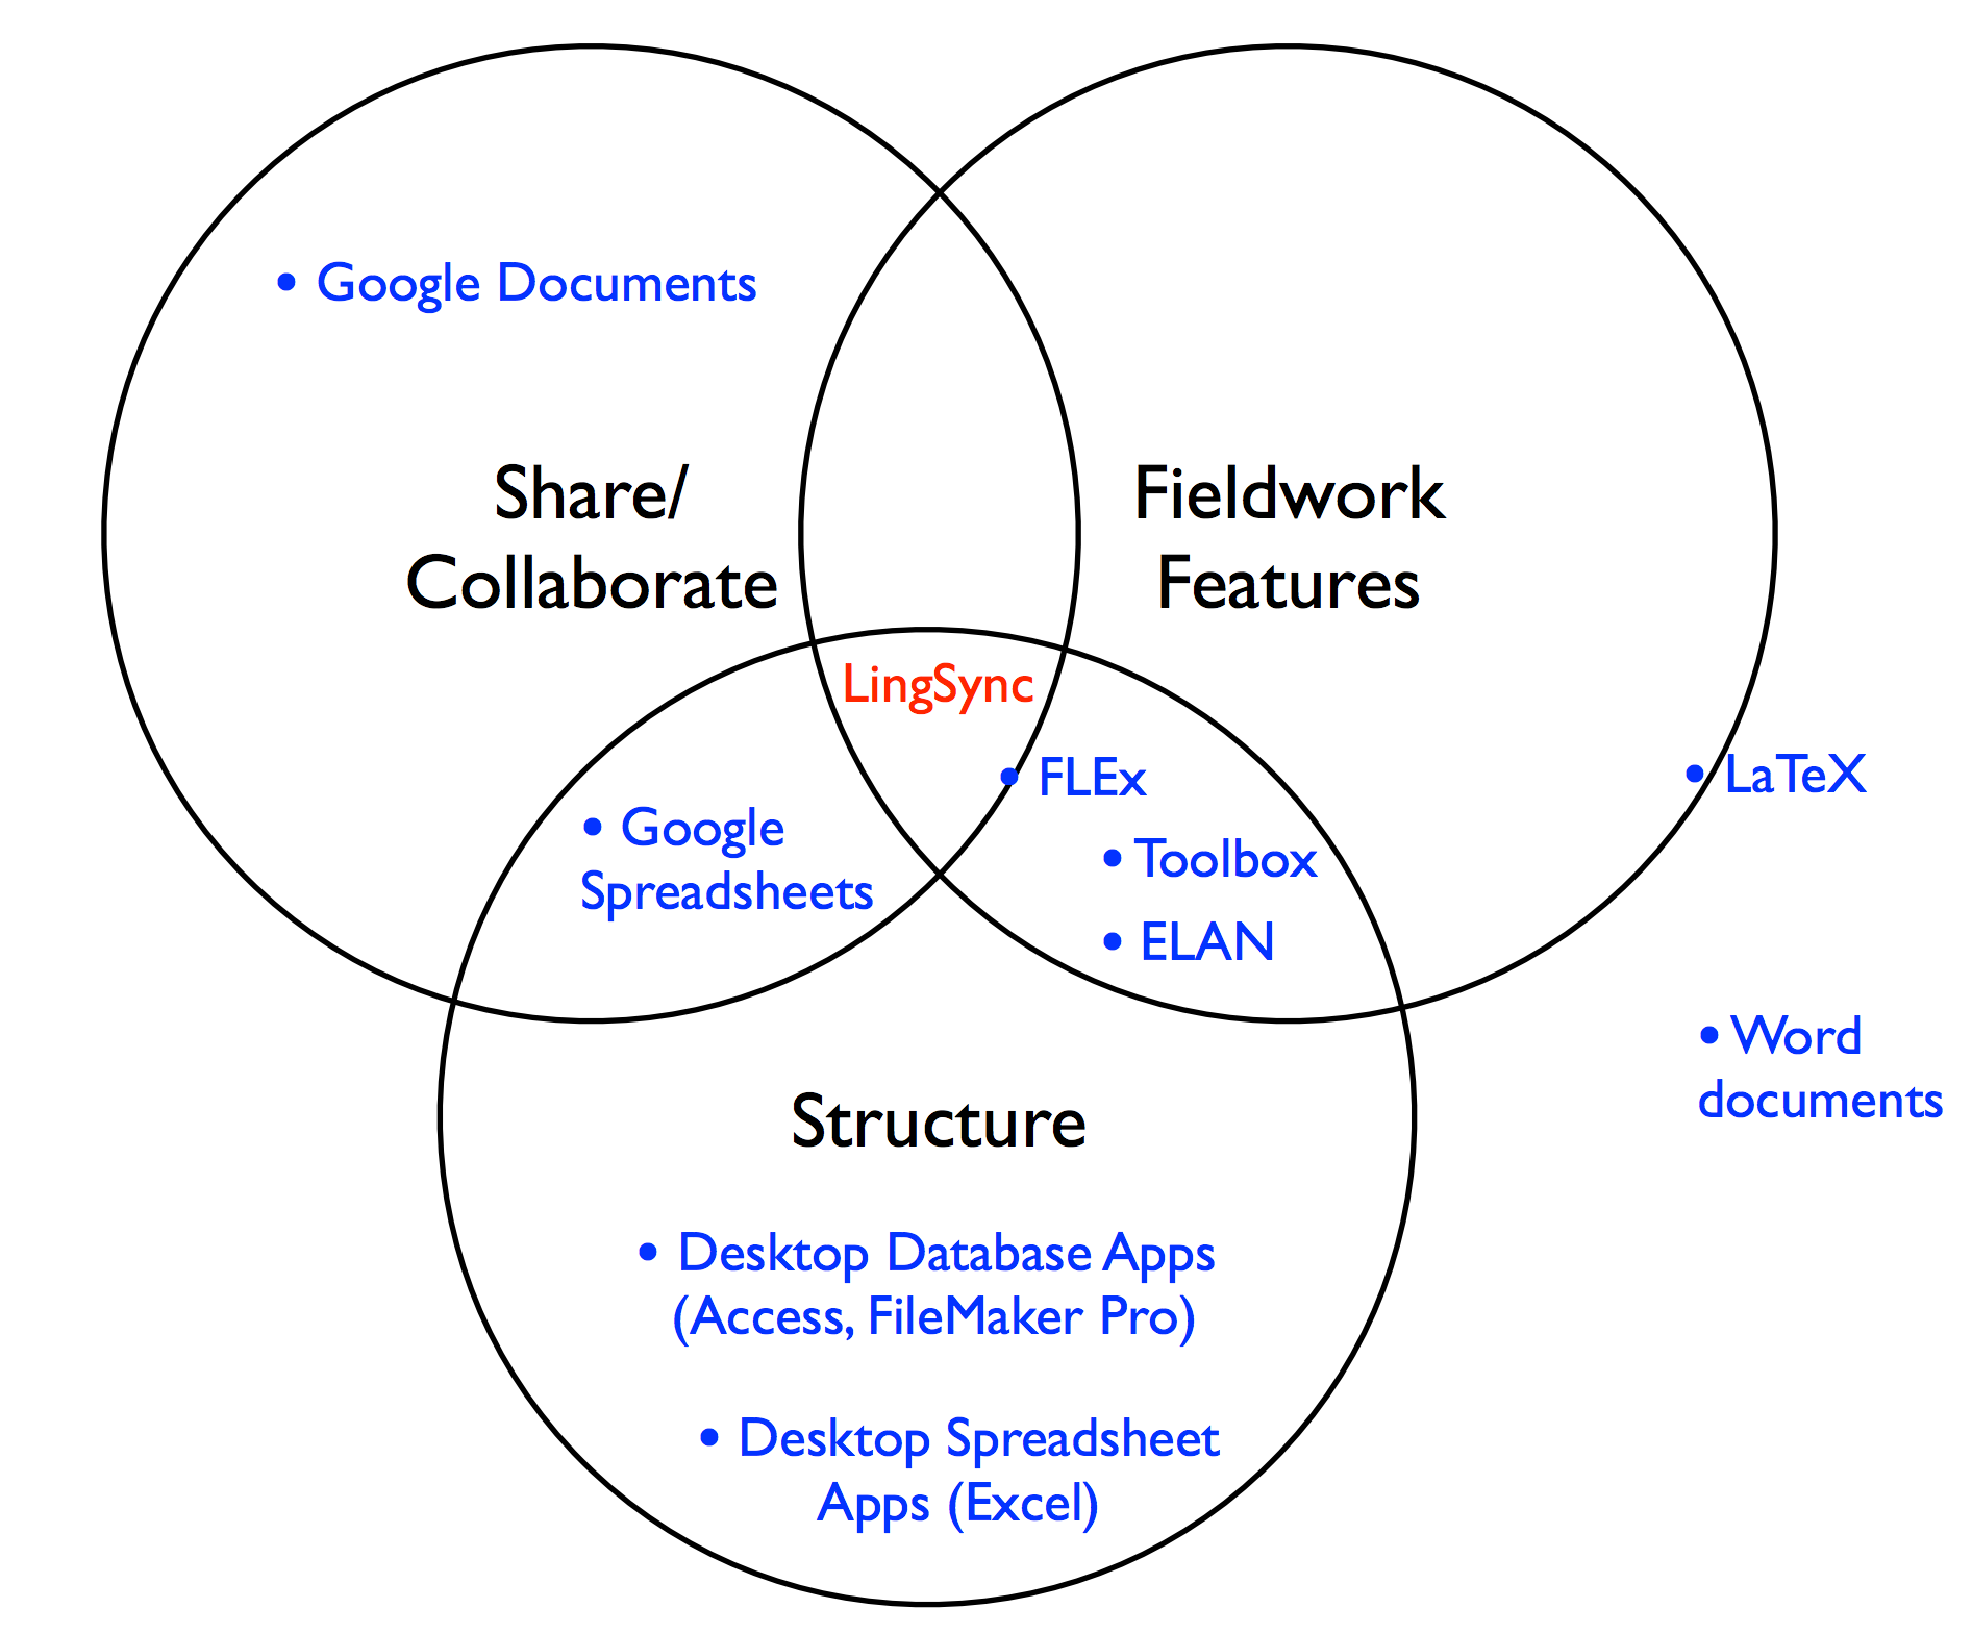
\includegraphics[width=3in]{../figures/other_software_sets}
\label{othersoftware}
\end{center}
\end{figure}

\end{frame}


\begin{frame}
%TODO will convert into latex diagrams once we are sure we want it.
\begin{figure}
\begin{center}
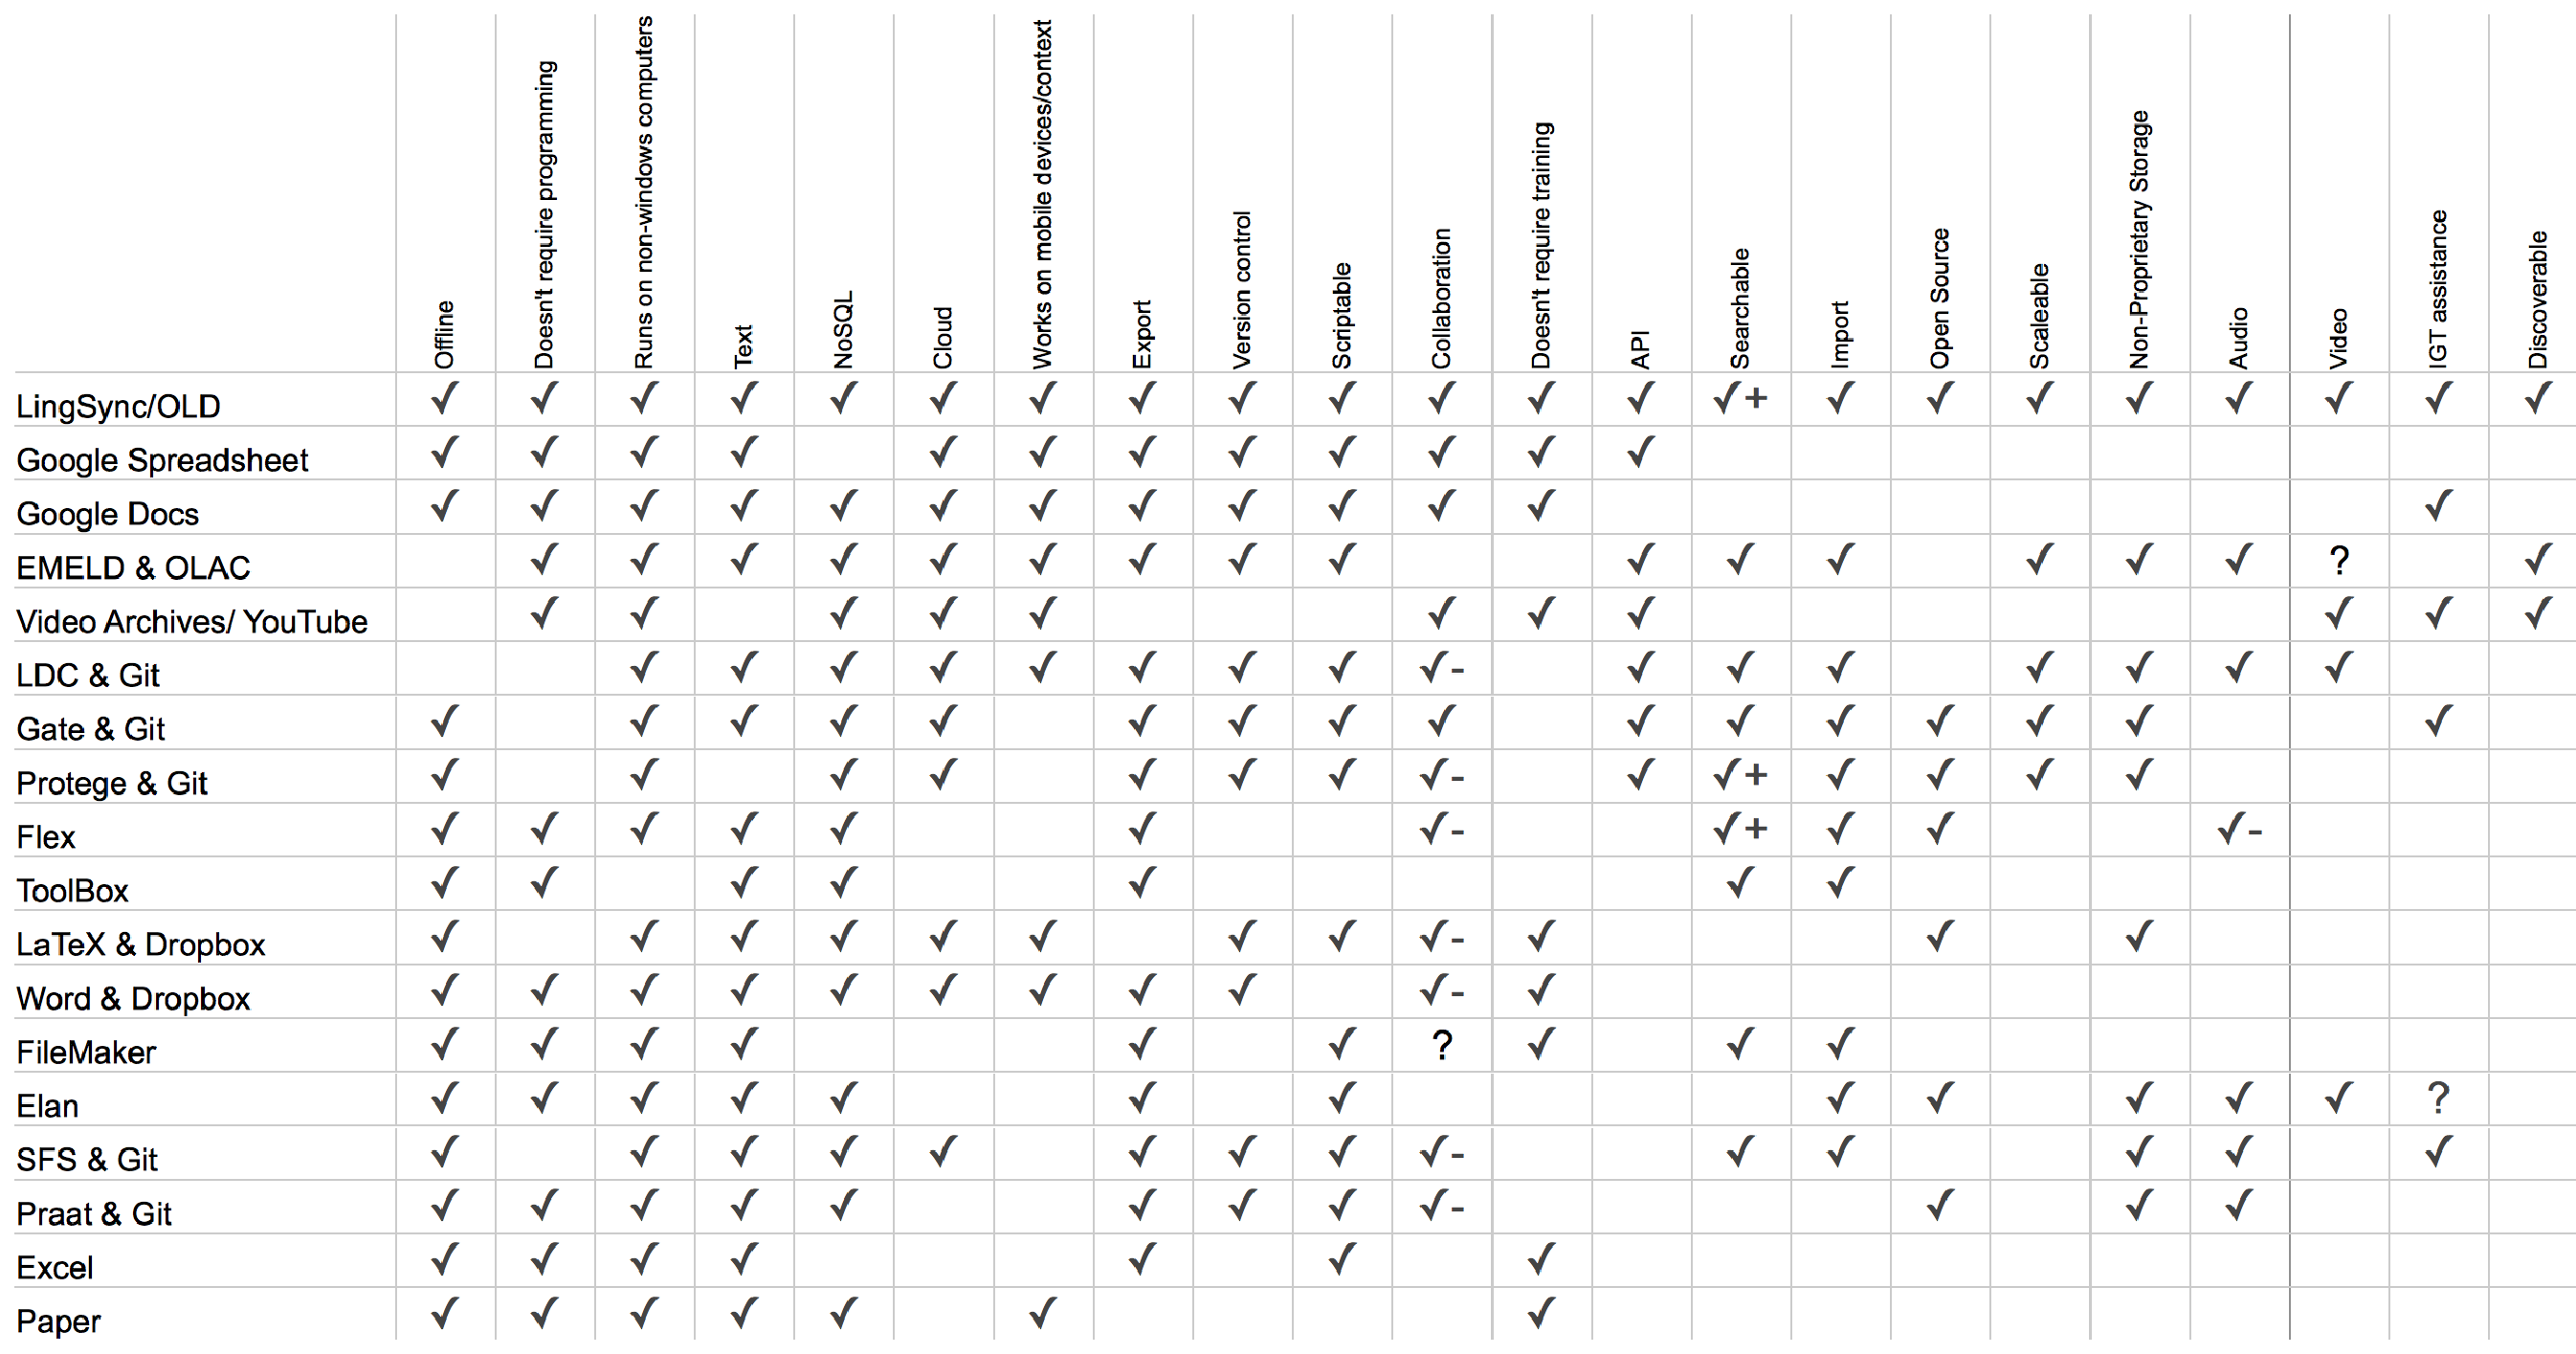
\includegraphics[width=3in]{../figures/other_software}
\caption{Many ad-hoc software combinations are used by teams.}
\label{allothersoftware}
\end{center}
\end{figure}
\end{frame}


\section[LingSync/OLD]{New models for data collection and management}
\subsection{LingSync}\label{sec:lingsync}


\begin{frame}
%TODO will convert into latex diagrams once we are sure we want it.
\begin{figure}
\begin{center}
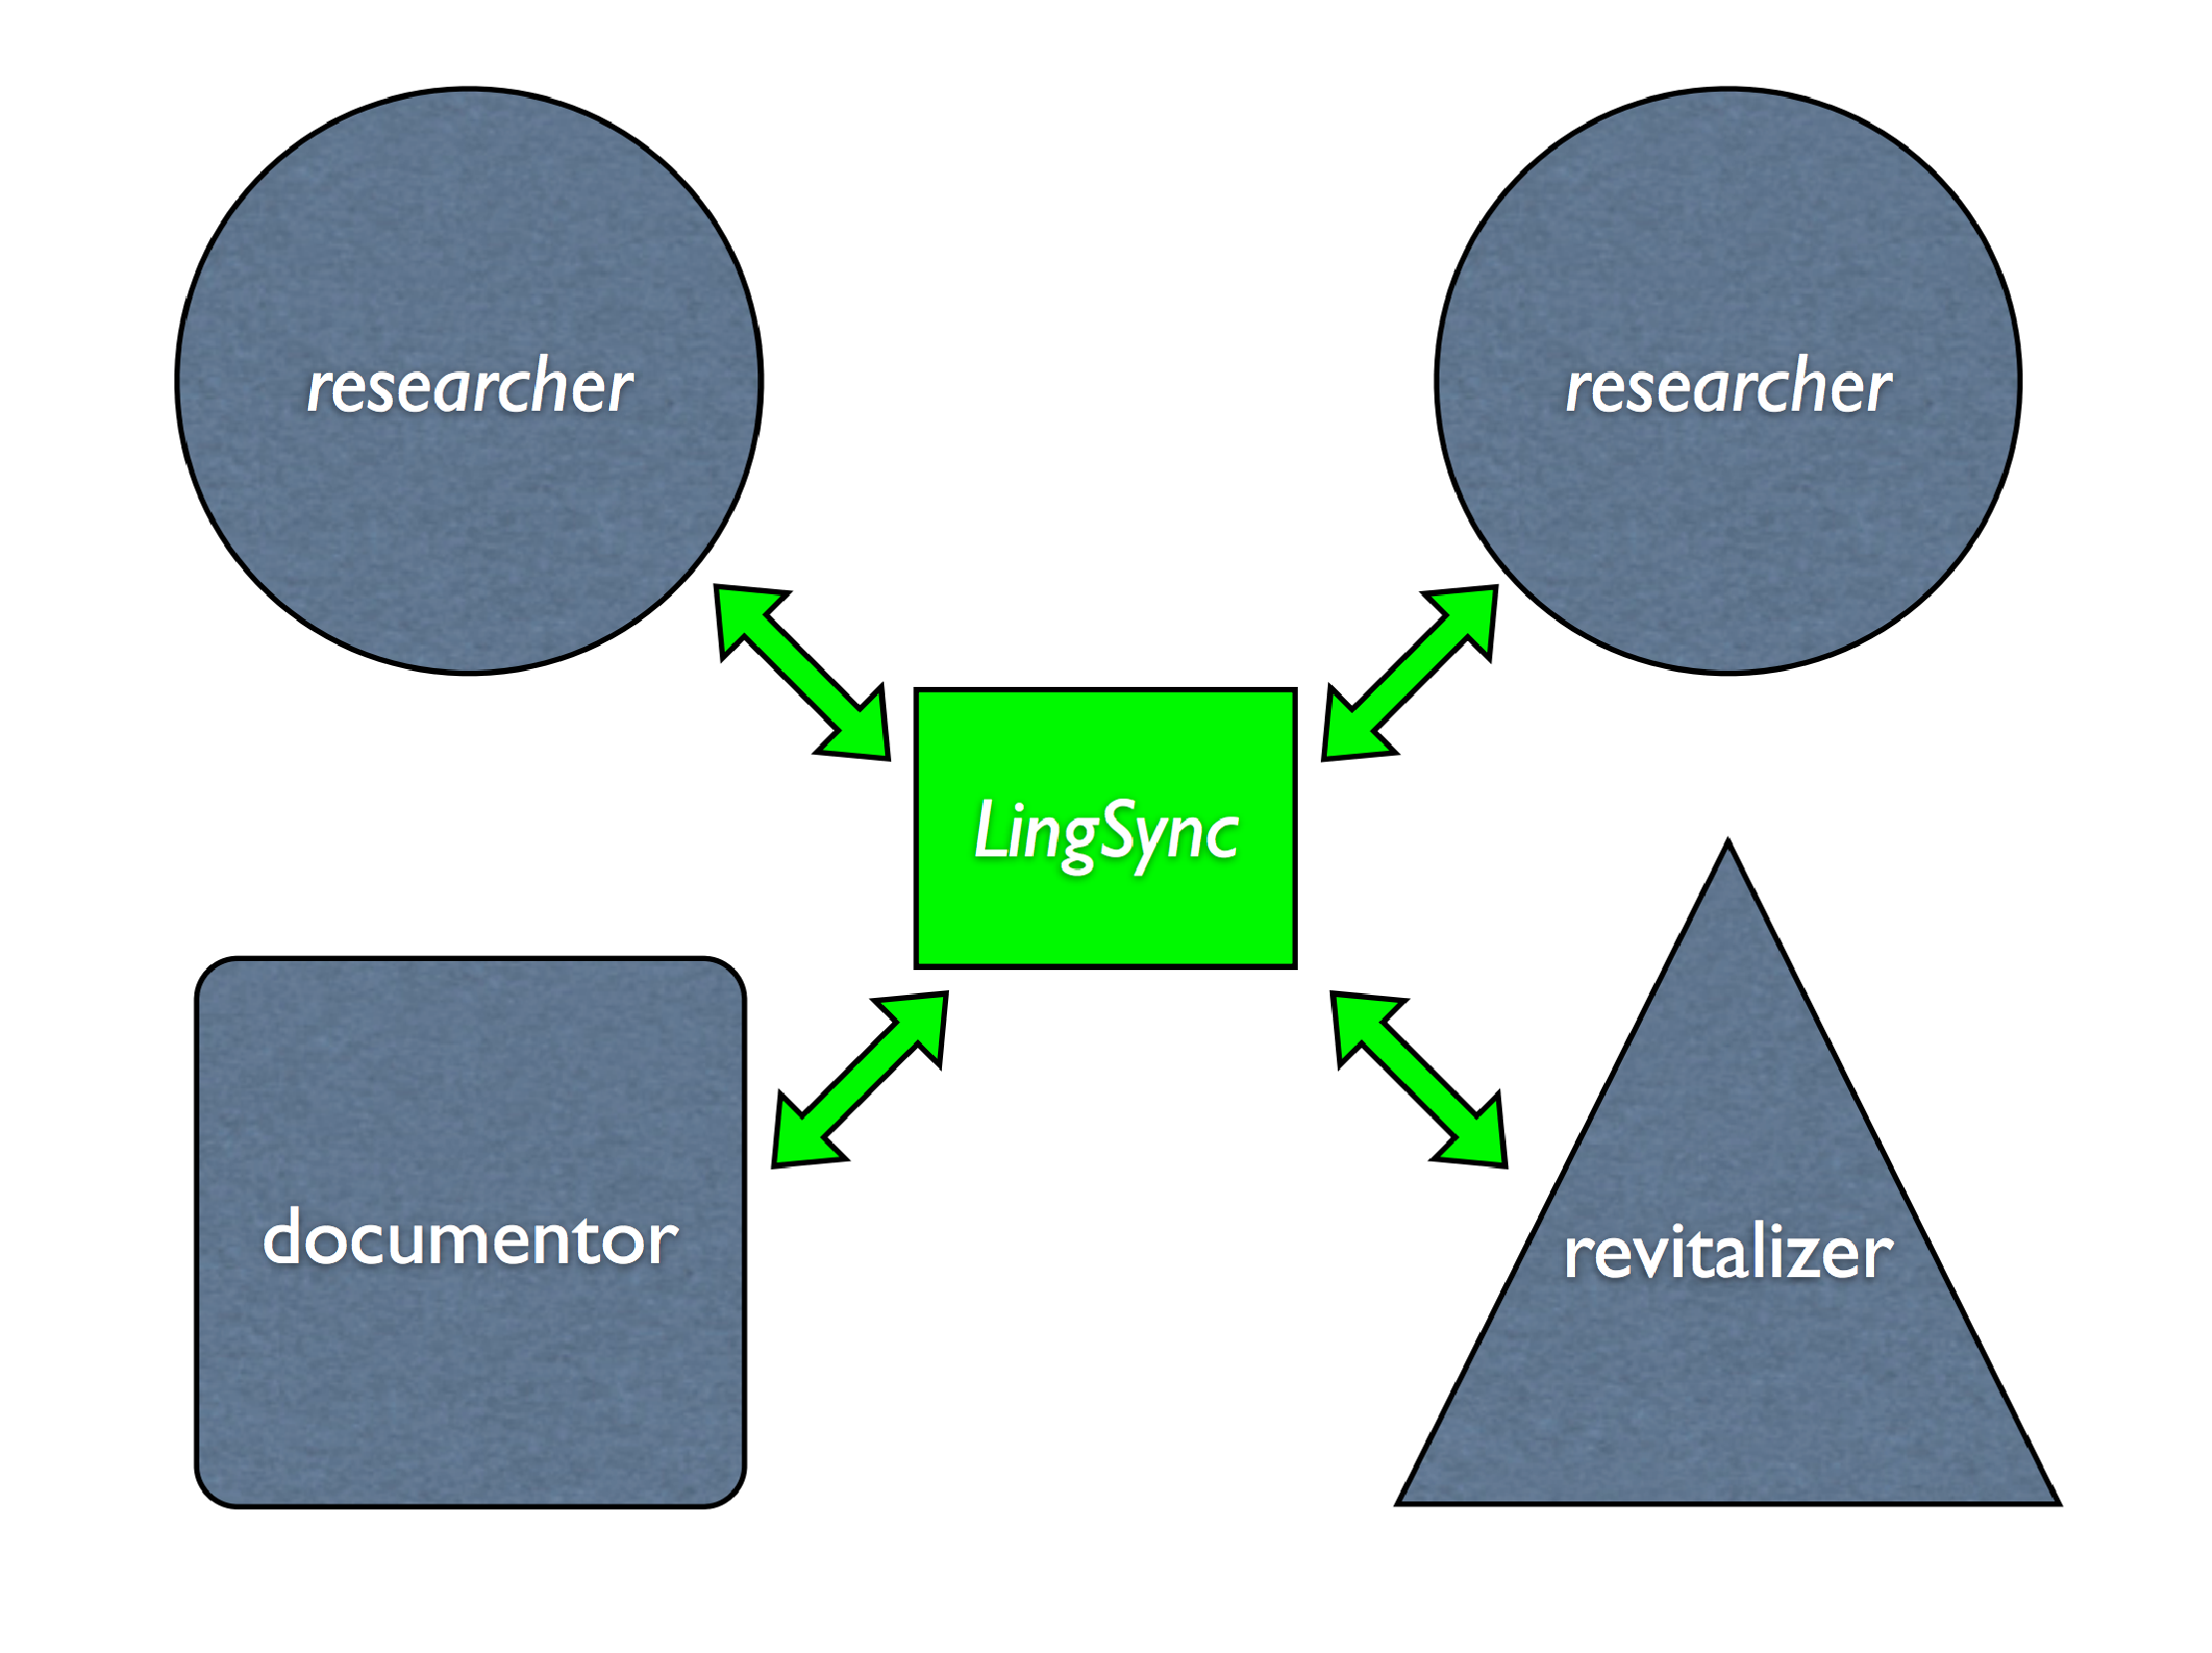
\includegraphics[width=3in]{../figures/bridge_stakeholders}
\label{lingsync:bridge}
\end{center}
\end{figure}
\end{frame}



\begin{frame}
%TODO will convert into latex diagrams once we are sure we want it.
\begin{figure}
\begin{center}
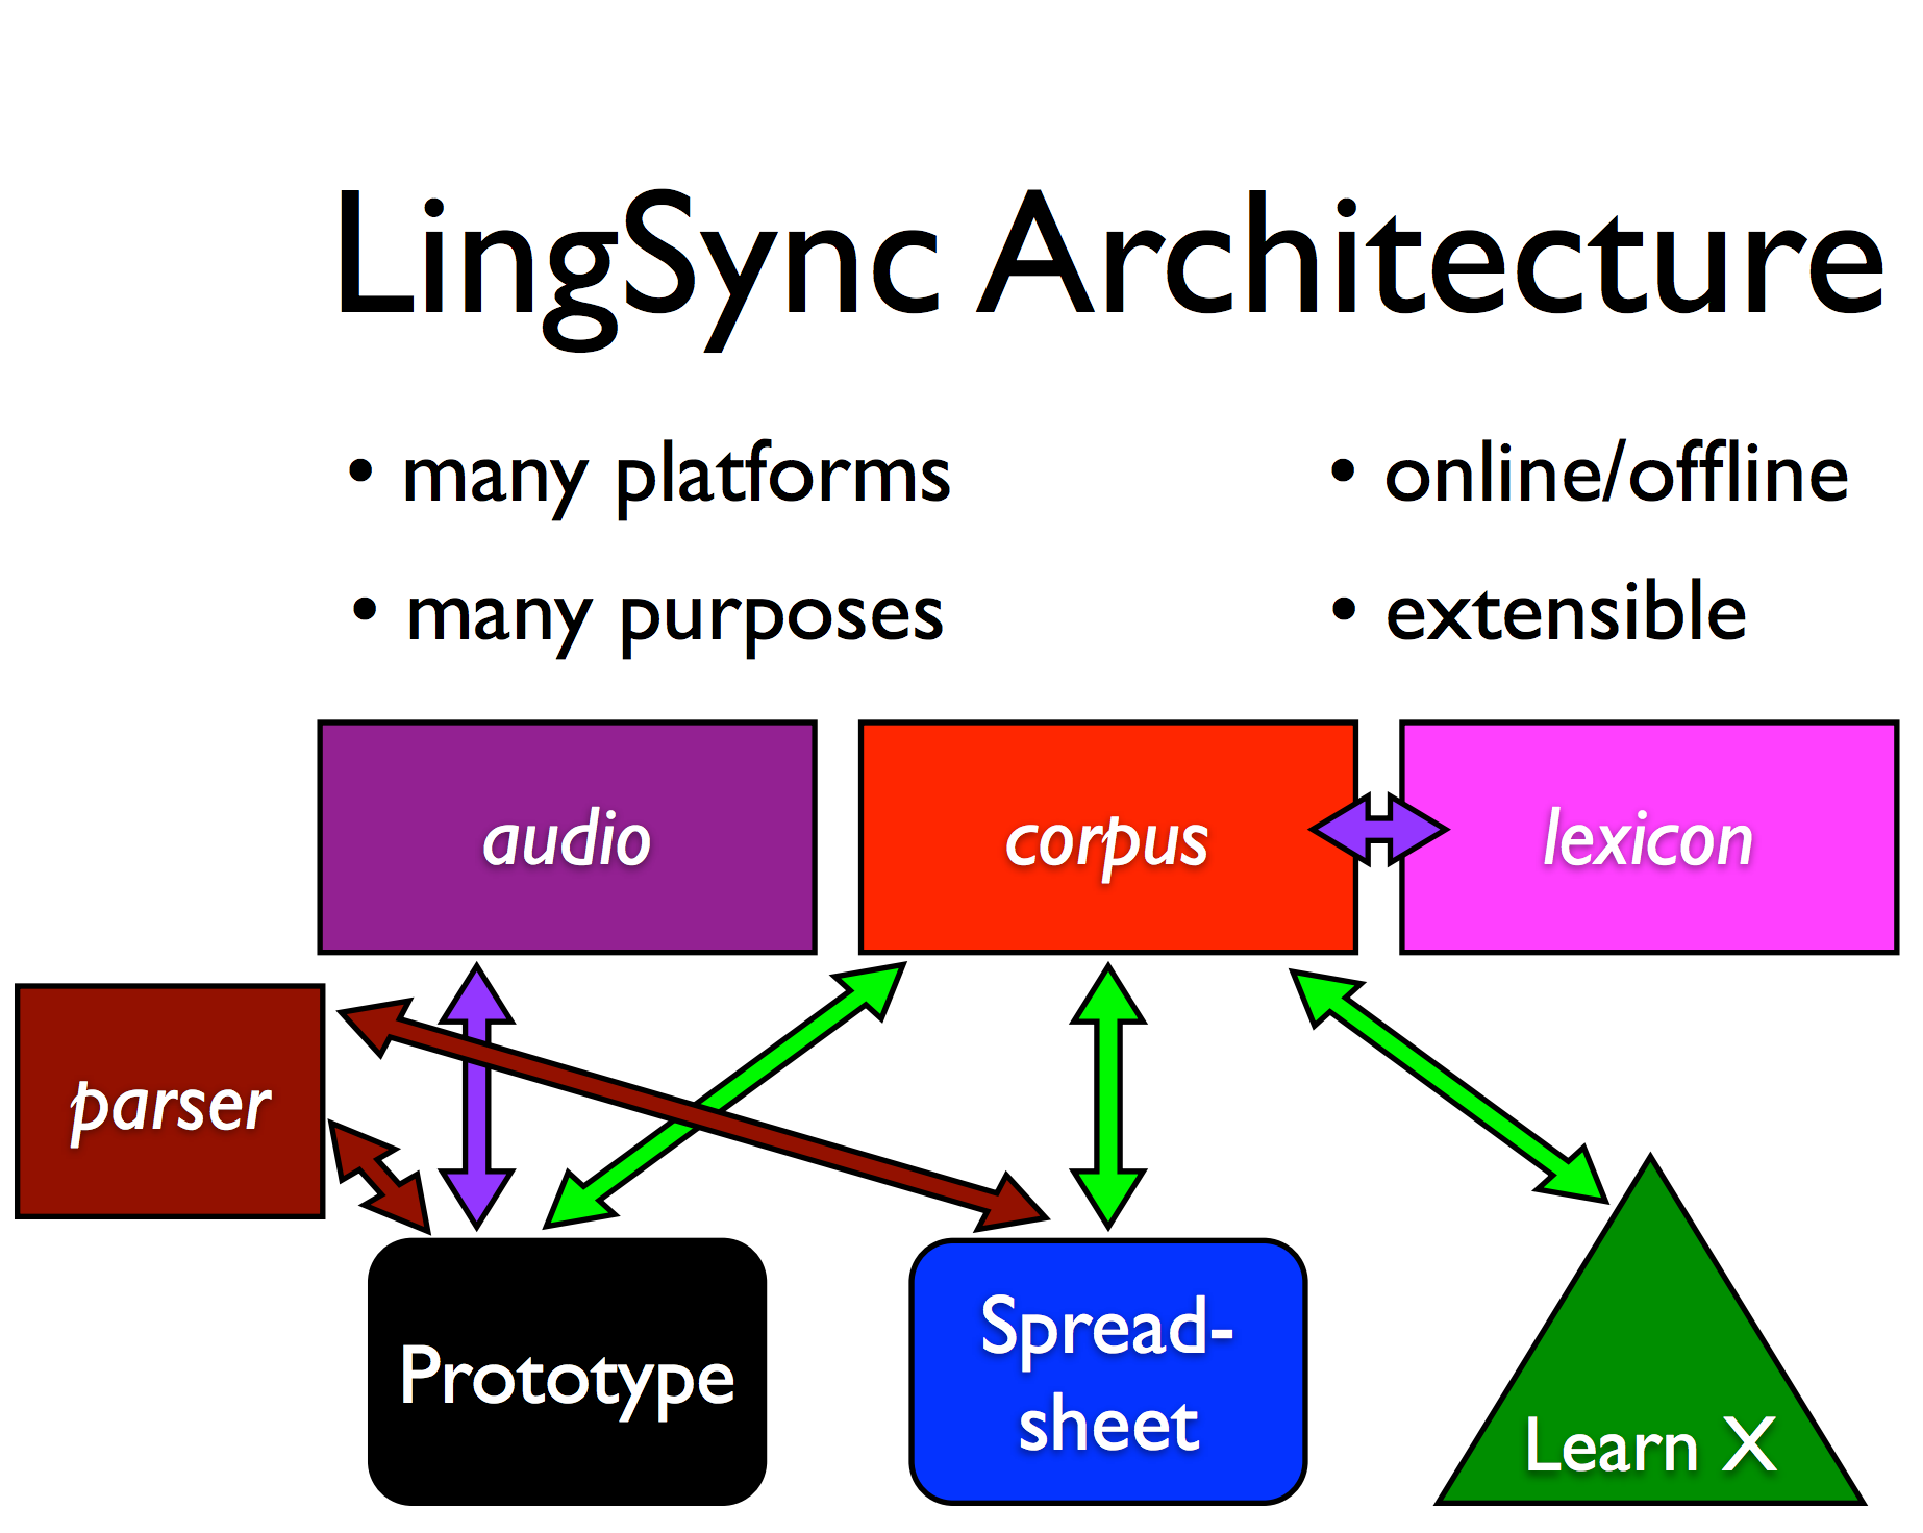
\includegraphics[width=3in]{../figures/architecture}
\label{lingsync:architecture}
\end{center}
\end{figure}
\end{frame}


\begin{frame}
%TODO will convert into latex diagrams once we are sure we want it.
\begin{figure}
\begin{center}
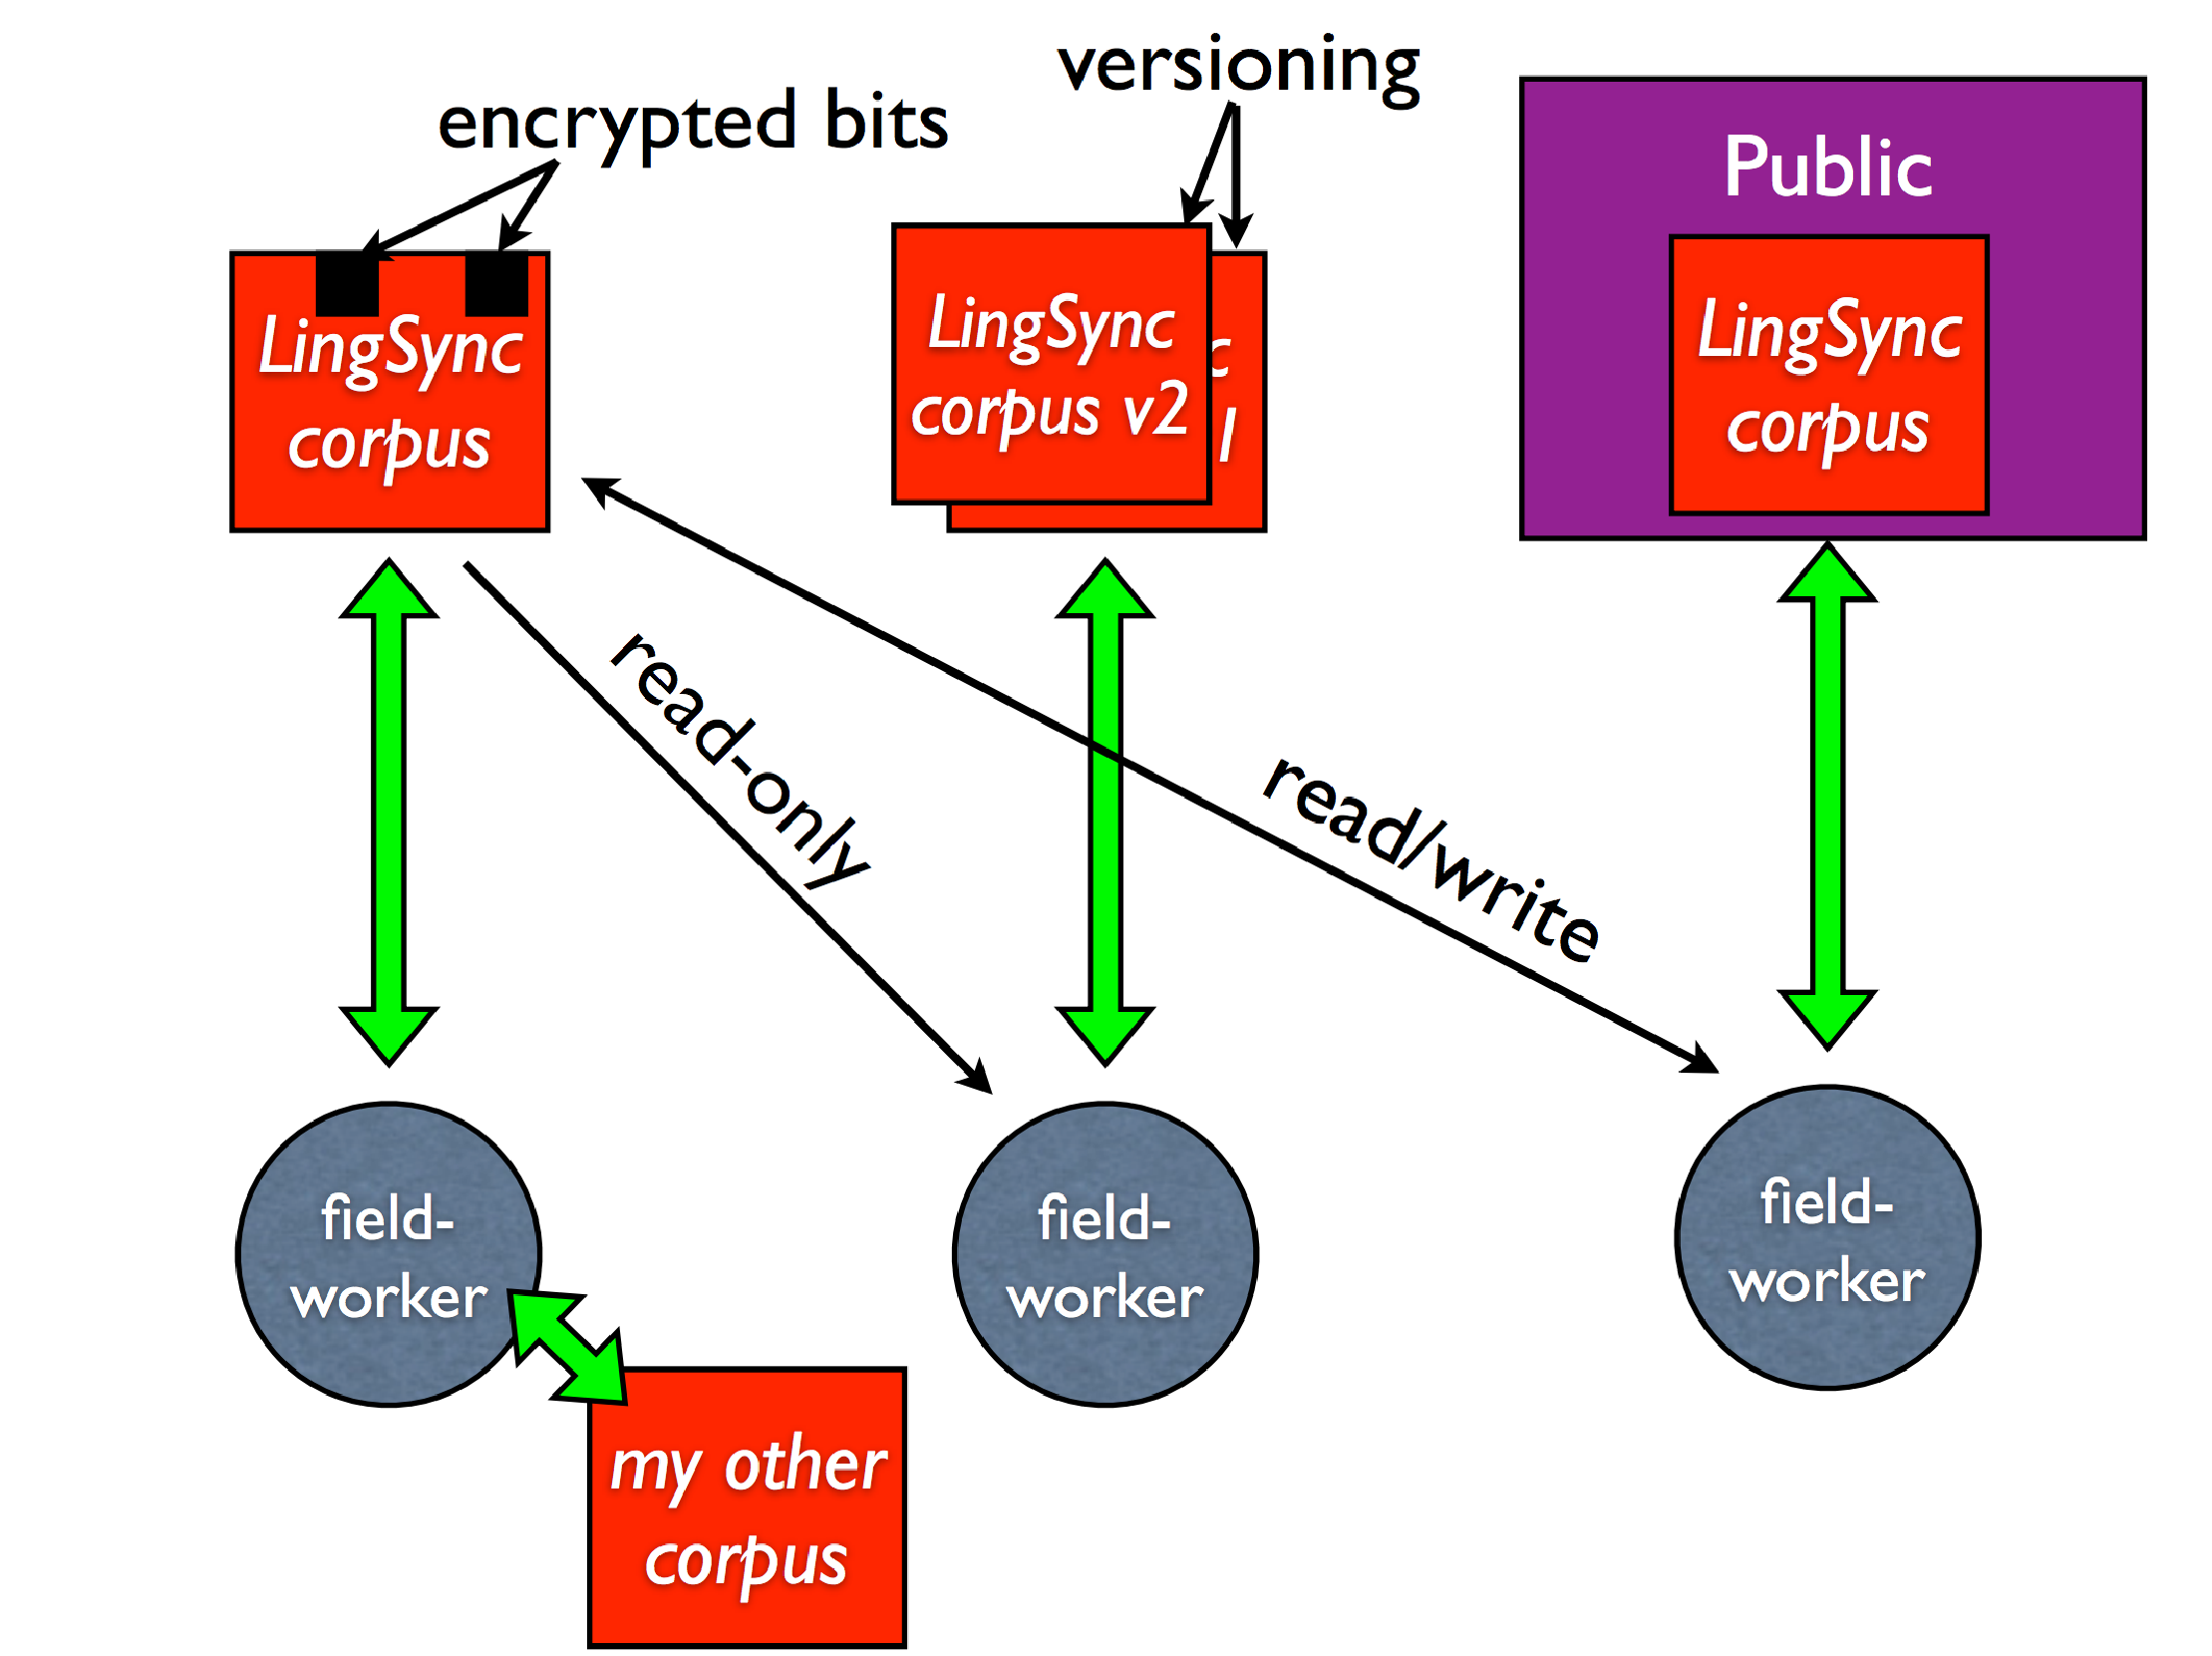
\includegraphics[width=3in]{../figures/corpora}
\label{lingsync:corpora}
\end{center}
\end{figure}
\end{frame}

\subsection{OLD}\label{sec:old}

\begin{frame}
OLD
\end{frame}

%\subsection{LingSync/OLD}

\subsection{User adoption}

\begin{frame}
User adoption
\end{frame}


%\section[Data]{Using LingSync/OLD}\label{open-data}
%
%\begin{frame}
%Using LingSync/OLD
%\end{frame}


\section[Plugins]{Plugins \& Reusing existing tools and libraries}

\subsection{Audio}
\subsubsection[Alignment]{Audio-transcription alignment}

\begin{frame}
Audio-transcription alignment
\end{frame}


\subsubsection[ASR]{Speech Recognition for Information Retrieval}

\begin{frame}
Speech Recognition for Legal Search in Kartuli
\end{frame}


\subsection{Morphology}



\subsubsection[Existing]{Existing morphological parsers}

\begin{frame}
Existing morphological parsers
\end{frame}




\subsubsection[Statistical]{Semi-supervised morphological parsers}

\begin{frame}
Semi-supervised morphological parsers
\end{frame}




\subsubsection[Novel]{Novel morphological parsers}

\begin{frame}
Novel morphological parsers
\end{frame}




\section{The Take-Home}

\begin{frame}
Take Home
\end{frame}

\section*{(Team)}

\begin{frame}
Acknowledgements
\end{frame}



\begin{frame}
References
\end{frame}


\end{document}
